\documentclass[12pt]{article}

\usepackage[utf8]{inputenc}
\usepackage{latexsym,amsfonts,amssymb,amsthm,amsmath}
\usepackage{tikz}
\usepackage{stanli}
\usetikzlibrary{shapes,calc,through,3d,patterns}
\usetikzlibrary{arrows.meta,decorations.pathreplacing,angles,quotes}
\usepackage{multicol}
\usepackage{geometry}
\usepackage{mathtools}
\usepackage{siunitx}
\usepackage{booktabs}

\setlength{\parindent}{0in}
\setlength{\oddsidemargin}{-0.25in}
\setlength{\textwidth}{7in}
\setlength{\textheight}{9.3in}
\setlength{\topmargin}{-1in}
\setlength{\headheight}{18pt}

\newcommand\blfootnote[1]{%
    \begingroup
    \renewcommand\thefootnote{}\footnote{#1}%
    \addtocounter{footnote}{-1}%
    \endgroup
}

\definecolor{darkred}{rgb}{0.6,0,0}

\newcommand{\bolddelta}{\boldsymbol\delta}
\newcommand{\boldxi}{\boldsymbol\xi}



\begin{document}

\noindent ME473 - Dynamic finite element analysis of structures\hfill EPFL\\
Stefano Burzio \hfill 2025\\
\vspace{0.3cm}

\hspace*{\fill}\textbf{\Large Problem set 8 - solutions}\hspace*{\fill}

\hrulefill

\subsection*{Problem 1}
The plate is discretized using a structured mesh of \(2 \times 2\) bilinear quadrilateral elements, resulting in a total of 9 nodes. Each node \(\mathbf{x}_i\) (\(i = 1, \dots, 9\)) is associated with three degrees of freedom (DOFs): the transverse displacement \(d^i\), and the rotations \(\theta_1^i\) and \(\theta_2^i\) about the \(x\)- and \(y\)-axes, respectively. The total number of DOFs in the discretized system is therefore 27. We shall identify the set of free DOFs corresponding to three distinct boundary conditions.

\paragraph*{1. Clamped on all four edges}
The transverse displacement and both rotations are fully restrained on all edges. Mathematically, the constraints are expressed as:
\[
    d = 0, \quad \theta_1 = 0, \quad \theta_2 = 0 \quad \text{on all boundary nodes}.
\]

The nodes located on the boundary of the plate are:
\[
    \mathbf{x}_1, \mathbf{x}_2, \mathbf{x}_3, \mathbf{x}_4, \mathbf{x}_6, \mathbf{x}_7, \mathbf{x}_8, \mathbf{x}_9,
\]
amounting to 8 nodes. Each contributes 3 constrained DOFs, yielding a total of \(24\) constrained DOFs. The only unconstrained (free) degrees of freedom are those associated with the interior node \(\mathbf{x}_5\):
\[
    d^5, \quad \theta_1^5, \quad \theta_2^5.
\]

\paragraph*{2. Simply supported on horizontal edges and free on vertical edges} For a simply supported edge in Reissner--Mindlin theory, the transverse displacement and the rotation normal to the edge are constrained. For horizontal edges, this yields:
\[
    d = 0, \quad \theta_2 = 0.
\]

The affected nodes on the bottom and top horizontal edges are:
\[
    \mathbf{x}_1, \mathbf{x}_4, \mathbf{x}_7 \quad \text{(bottom edge)}, \qquad \mathbf{x}_3, \mathbf{x}_6, \mathbf{x}_9 \quad \text{(top edge)}.
\]

Each of these 6 nodes has 2 constrained DOFs (\(d\) and \(\theta_2\)), resulting in \(12\) constrained DOFs. The constrained DOFs are:
\[
    \begin{aligned}
         & d^1, \theta_2^1, \quad d^4, \theta_2^4, \quad d^7, \theta_2^7, \\
         & d^3, \theta_2^3, \quad d^6, \theta_2^6, \quad d^9, \theta_2^9.
    \end{aligned}
\]
The remaining 15 DOFs are unconstrained and therefore free.

\paragraph*{3. Corner nodes simply supported} Assuming the simplest interpretation consistent with the application, each corner node is constrained in transverse displacement only: $d = 0$. The corner nodes are:
\[
    \mathbf{x}_1, \mathbf{x}_3, \mathbf{x}_7, \mathbf{x}_9.
\]
Each of these nodes has $1$ constrained DOFs, giving a total of \(4\) constrained DOFs. The constrained DOFs are:
\[ d^1, d^3, d^7, d^9,
\]

The remaining 23 DOFs, associated with the edge midpoints, rotations at the corners and the interior node, are free.

\paragraph*{Comparison of fundamental frequencies}
The first fundamental frequency of a vibrating plate depends strongly on the stiffness of the system, which is determined by the type and extent of the applied boundary conditions. A stiffer system resists deformation more effectively and thus exhibits higher natural frequencies. Conversely, a system with greater flexibility (i.e., fewer constraints) will have lower frequencies.


The first configuration imposes the most restrictive boundary conditions as all three local degrees of freedom (transverse displacement and both rotations) are fully constrained along every edge. This yields the maximum structural stiffness and therefore the highest natural frequencies.

The second and the third case are fairly similar in terms of the is the first fundamental frequency. In the third case, their location at the corners provides localized stiffness. Compared to case 2, this configuration may offer slightly smaller resistance to deformation, especially far from the corners.

Based on the relative flexibility of each configuration, we expect the following qualitative ordering of the first fundamental frequencies:
\[
    \omega_1^{\text{(corners simply supported)}} < \omega_1^{\text{(free + simply supported)}} < \omega_1^{\text{(fully clamped)}}.
\]

\subsection*{Problem 2}
Since the plate is discretized using a single bilinear plate element, the global and element mass and stiffness matrices are identical; hence, no assembly procedure is required. Furthermore, because the reference, element, and archetypal domains coincide, i.e., $\Omega = {}^e\Omega = {}^a\Omega$, the local coordinates $\xi_1$, $\xi_2$ and the global coordinates $x$, $y$ can be used interchangeably, i.e., $\partial_x=\partial_{\xi_1}$ and $\partial_y=\partial_{\xi_2}$.

Under these conditions, the consistent mass matrix takes the form
\begin{align*}
    \mathbf M & =\int_{\Omega}\, {}^a\mathbf H^T\, \mathbf I\, {}^a\mathbf H \, d\Omega                                                               \\
              & = \int_{-1}^1\int_{-1}^1 \begin{bmatrix}
                                             {}^a h_1^2 \mathbf I & {}^a h_1{}^a h_2 \mathbf I & {}^a h_1{}^a h_3 \mathbf I & {}^a h_1{}^a h_4 \mathbf I  \\
                                                                  & {}^a h_2^2 \mathbf I       & {}^a h_2{}^a h_3 \mathbf I & {}^a h_2{}^a h_4 \mathbf I  \\
                                                                  &                            & {}^a h_3^2 \mathbf I       & {}^a h_3 {}^a h_4 \mathbf I \\
                                             sym.                 &                            &                            & {}^a h_4^2 \mathbf I        \\
                                         \end{bmatrix} \, d\xi_2d\xi_1
\end{align*}
Analogously, the global stiffness matrix is given by $\mathbf{K} = \mathbf{K}_b + \mathbf{K}_s$, where the bending contribution is expressed as
\begin{align*}
    \mathbf K_b & =\int_{\Omega}\mathbf B_b^T\overline{\boldsymbol{C}_b}\mathbf B_b\, d\Omega                                                                                                                                                                        \\
                & =\frac{h^3}{12}\int_{-1}^1\int_{-1}^1\begin{bmatrix}
                                                           (\nabla_b{}^a h_1)^T \mathbf C_b \nabla_b{}^a h_1 & (\nabla_b{}^a h_1)^T \mathbf C_b \nabla_b{}^a h_2 & (\nabla_b{}^a h_1)^T \mathbf C_b \nabla_b{}^a h_3 & (\nabla_b{}^a h_1)^T\mathbf C_b \nabla_b{}^a h_4  \\
                                                                                                             & (\nabla_b{}^a h_2)^T \mathbf C_b \nabla_b{}^a h_2 & (\nabla_b{}^a h_2)^T \mathbf C_b \nabla_b{}^a h_3 & (\nabla_b{}^a h_2)^T \mathbf C_b \nabla_b{}^a h_4 \\
                                                                                                             &                                                   & (\nabla_b{}^a h_3)^T \mathbf C_b \nabla_b{}^a h_3 & (\nabla_b{}^a h_3)^T\mathbf C_b \nabla_b{}^a h_4  \\
                                                           sym.                                              &                                                   &                                                   & (\nabla_b{}^a h_4)^T \mathbf C_b \nabla_b{}^a h_4 \\
                                                       \end{bmatrix} \, d\xi_2d\xi_1
\end{align*}
where $\nabla_b$ denotes the bending strain-displacement operator. The shear contribution is similarly given by
$$\mathbf K_s =\int_{\Omega}\mathbf B_s^T\overline{\boldsymbol{C}_s}\mathbf B_s\, d\Omega$$
where $\mathbf{C}_s$ replaces $\mathbf{C}_b$, and $\nabla_s$ replaces  $\nabla_b$, reflecting the different nature of the strain measures in the shear formulation.

The boundary conditions enforce zero transverse displacements and rotations at all nodes except $\mathbf{x}_1$, which remains free. As a result, the free degrees of freedom correspond to the first three rows and columns of the global matrices. The reduced mass matrix is then
\begin{align*}
    \mathbf M^{red} & = \int_{-1}^1\int_{-1}^1 {}^a h_1^2 \mathbf I \, d\xi_2d\xi_1                         \\
                    & =\int_{-1}^1\int_{-1}^1 {}^a h_1^2 \, d\xi_2d\xi_1 \begin{bmatrix}
                                                                             \rho h & 0           & 0           \\
                                                                             0      & \rho h^3/12 & 0           \\
                                                                             0      & 0           & \rho h^3/12 \\
                                                                         \end{bmatrix} \\
                    & = \frac{4}{9}\begin{bmatrix}
                                       \rho h & 0           & 0           \\
                                       0      & \rho h^3/12 & 0           \\
                                       0      & 0           & \rho h^3/12 \\
                                   \end{bmatrix}
\end{align*}
The corresponding reduced stiffness matrix is decomposed as $\mathbf{K}^{\text{red}} = \mathbf{K}_b^{\text{red}} + \mathbf{K}_s^{\text{red}}$, with
$$ \mathbf K^{red}_b = \frac{h^3}{12}\int_{-1}^1\int_{-1}^1 (\nabla_b{}^a h_1)^T \mathbf C_b \nabla_b{}^a h_1\, d\xi_2d\xi_1$$
Substituting the expressions for $\mathbf{C}_b$ and $\nabla_b$, this becomes
$$\mathbf K^{red}_b=\frac{Eh^3}{12(1 - \nu^2)}\int_{-1}^1\int_{-1}^1 \begin{bmatrix}
        0                  & 0                   & 0                   \\
        0                  & -\partial_y{}^a h_1 & -\partial_x{}^a h_1 \\
        \partial_x{}^a h_1 & 0                   & \partial_y{}^a h_1  \\
    \end{bmatrix}\begin{bmatrix}
        1   & \nu & 0                 \\
        \nu & 1   & 0                 \\
        0   & 0   & \frac{1 - \nu}{2}
    \end{bmatrix}\begin{bmatrix}
        0 & 0                   & \partial_x{}^a h_1 \\
        0 & -\partial_y{}^a h_1 & 0                  \\
        0 & -\partial_x{}^a h_1 & \partial_y{}^a h_1 \\
    \end{bmatrix}\, d\xi_2d\xi_1 $$
Which simplify and evaluates to
\begin{align*}
    \mathbf K^{red}_b & =D\int_{-1}^1\int_{-1}^1 \begin{bmatrix}
                                                     0 & 0                                                        & 0                                                        \\[5pt]
                                                     0 & (\partial_y h_1)^2 + \frac{1 - \nu}{2}(\partial_x h_1)^2 & -\frac{1 + \nu}{2}\partial_x h_1 \partial_y h_1          \\[5pt]
                                                     0 & -\frac{1 + \nu}{2}\partial_x h_1 \partial_y h_1          & (\partial_x h_1)^2 + \frac{1 - \nu}{2}(\partial_y h_1)^2
                                                 \end{bmatrix}\, d\xi_2d\xi_1 \\
                      & =D\begin{bmatrix}
                              0 & 0                 & 0                 \\
                              0 & 1/3 + (1 - \nu)/6 & -(1 + \nu)/8      \\
                              0 & -(1 + \nu)/8      & 1/3 + (1 - \nu)/6
                          \end{bmatrix}
\end{align*}
Recall that the flexural rigidity of the plate is $D = \frac{E h^3}{12(1-\nu^2)}$.
For the shear contribution, we have
$$ \mathbf K^{red}_s  = h\int_{-1}^1\int_{-1}^1 (\nabla_s{}^a h_1)^T \mathbf C_s \nabla_s{}^a h_1\, d\xi_2d\xi_1 $$
Substituting the expressions for $\mathbf{C}_s$ and $\nabla_s$, this becomes
\begin{align*}
    \mathbf K^{red}_s & =Gkh\int_{-1}^1\int_{-1}^1 \begin{bmatrix}
                                                       \partial_x{}^a h_1 & \partial_y{}^a h_1 \\
                                                       0                  & -{}^a h_1          \\
                                                       {}^a h_1           & 0
                                                   \end{bmatrix}\begin{bmatrix}
                                                                    1 & 0 \\                                                                                      0 & 1 \\                                                                                    \end{bmatrix}\begin{bmatrix}
                                                                                                                                                                                                                                                                           \partial_x{}^a h_1 & 0         & {}^a h_1 \\
                                                                                                                                                                                                                                                                           \partial_y{}^a h_1 & -{}^a h_1 & 0        \\
                                                                                                                                                                                                                                                                       \end{bmatrix}\, d\xi_2d\xi_1 \\
                      & =Gkh\int_{-1}^1\int_{-1}^1 \begin{bmatrix}
                                                       (\partial_x h_1)^2 + (\partial_y h_1)^2 & -h_1 \partial_y h_1 & h_1 \partial_x h_1 \\
                                                       -h_1 \partial_y h_1                     & h_1^2               & 0                  \\
                                                       h_1 \partial_x h_1                      & 0                   & h_1^2
                                                   \end{bmatrix}   \, d\xi_2d\xi_1                                                                                                                                                                            \\
                      & = Gkh\begin{bmatrix}
                                 2/3  & 1/3 & -1/3 \\
                                 1/3  & 4/9 & 0    \\
                                 -1/3 & 0   & 4/9
                             \end{bmatrix}
\end{align*}
Recall that, for isotropic materials, the shear modulus $G$ is related to Young’s modulus $E$ and Poisson’s ratio $\nu$ by: $G = \frac{E}{2(1 + \nu)}$.


\subsection*{Problem 3}
The \texttt{MATLAB} code performs the computation of the fundamental natural frequency of a simply supported isotropic square plate with in-plane dimensions $1 \times 1$, where the plate thickness varies according to the values specified in the vector \texttt{h\_values}.

\textbf{Plate geometry}
\begin{verbatim}
length_X = 1; %length_X = 2a
length_Y = 1; %length_Y = 2b  

h_values = [0.01 0.02 0.05 0.075 0.1 0.125 0.15 0.5 1];
\end{verbatim}
\textbf{Material properties}
\begin{verbatim}
E = 10920;
nu = 0.3; 
rho = 1;
kappa = 5/6; 
\end{verbatim}
\textbf{Material Mesh}

Generate structured rectangular mesh of bilinear elements by using the function \texttt{createRectangularMesh}.
\begin{verbatim}
number_elements_X = 8;
number_elements_Y = 8;

number_elements = number_elements_X * number_elements_Y;
number_nodes = (number_elements_X + 1) * (number_elements_Y + 1); 

number_of_nodes_per_element = 4;
number_of_dofs_per_node = 3;

number_dofs_per_element = number_of_nodes_per_element*number_of_dofs_per_node;
number_dofs = number_nodes*number_of_dofs_per_node;

[nodes, connectivity] = create_mesh(number_elements_X,number_elements_Y, 
        length_X, length_Y);
\end{verbatim}
\textbf{Boundary conditions}
Use the function \texttt{getConstrainedDOFs\_SSSS} to select the constrained DOFs for the specified boundary conditions: simply supported on all four edges.

\begin{verbatim}
constrained_dofs = getConstrainedDOFs_SSSS(number_elements_X, number_elements_Y, 
        'HTK');
\end{verbatim}

\textbf{Computation of the fundamental natural frequency for varying plate thickness values}

The next step involves the computation of the global stiffness matrix and global consistent mass matrix using helper functions (\texttt{formStiffnessThickPlate} and \texttt{formMassThickPlate}). These matrices represent the elastic and inertial properties of the system, respectively, and are assembled in the global coordinate system based on the element-level contributions. Then we apply the boundary conditions and compute the fundamental frequency of the plates.

\begin{verbatim}
approx_fundamental_freq = zeros(1, length(h_values));

for i = 1:length(h_values)
    h = h_values(i);

    % Bending constitutive matrix
    C_bending = h^3 * E / (12 * (1 - nu^2)) * [1 nu 0; nu 1 0; 0 0 (1 - nu) / 2];
    % Shear constitutive matrix
    C_shear = kappa * h * E / (2 * (1 + nu)) * eye(2);
    % Inertia matrix
    Inertia_matrix = rho * [h, 0, 0; 0, h^3 / 12, 0; 0, 0, h^3 / 12];

    % Assemble global stiffness and mass matrices
    stiffness = formStiffnessThickPlate(nodes, connectivity,
            C_bending, C_shear, 'selective_int'););
    mass = formMassThickPlate(nodes, connectivity, Inertia_matrix);
    
    % Apply boundary conditions 
    stiffness_freeDofs = stiffness(free_dofs, free_dofs);
    mass_freeDofs = mass(free_dofs, free_dofs);
    
    % Compute smallest eigenvalue (fundamental frequency)
    eigenvalues = vpa(eig(inv(mass_freeDofs)*stiffness_freeDofs),4);
    approx_fundamental_freq(i) = vpa(sqrt(min(eigenvalues)) / (2*pi),4);
end
\end{verbatim}

\textbf{Exact fundamental frequency}

The exact fundamental frequency is computed using closed-form formula for simply supported square plate.

\begin{verbatim}
exact_fundamental_freq = zeros(1, length(h_values));

for i = 1:length(h_values)
    h = h_values(i);
    exact_fundamental_freq(i) = computeExactFreqsThickPlate(1, length_X, length_Y,
            h, nu, E, rho, kappa);
end
\end{verbatim}

\textbf{Comparative analysis of the fundamental frequencies}

This section of the code visualizes and compares the numerical and exact solutions of the fundamental frequency for a square plate with varying thickness, and then quantifies the error between them.

\begin{verbatim}
figure;
plot(h_values, exact_fundamental_freq, 'b-o', 'LineWidth', 2, 'MarkerSize', 6); 
hold on;
plot(h_values, approx_fundamental_freq, 'r--s', 'LineWidth', 2, 'MarkerSize', 6);
hold off;

xlabel('$h$ (plate thickness)', 'Interpreter', 'latex', 'FontSize', 14)
ylabel('Fundamental frequency', 'Interpreter', 'latex', 'FontSize', 14)
title('Exact vs. Approximate Fundamental Frequency vs. $h$', 'Interpreter',
         'latex', 'FontSize', 16)
legend({'Exact', 'Approximate'}, 'Interpreter', 'latex', 'Location', 'best', 
        'FontSize', 12)

grid on
axis tight
set(gca, 'FontSize', 12)
\end{verbatim}

\begin{center}
    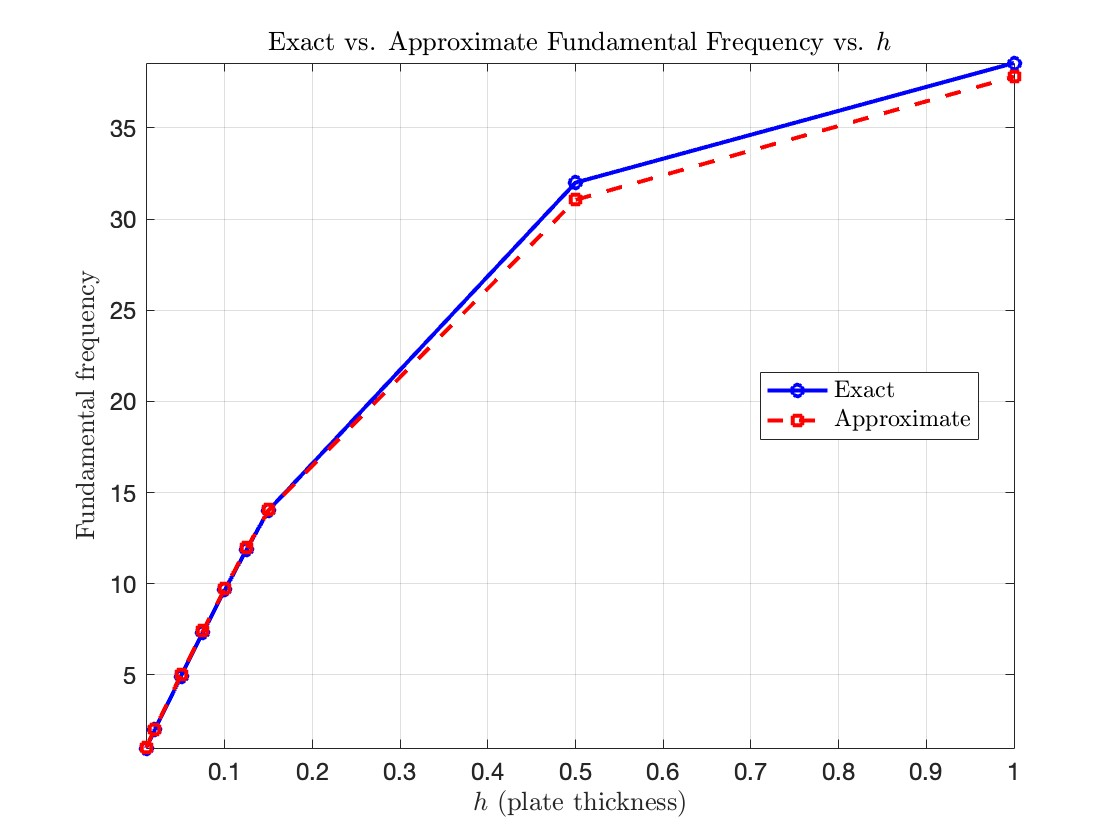
\includegraphics[width=7cm]{../images/freqThickPlates.jpg}
\end{center}

\begin{verbatim}
% Compute relative error as a percentage
relative_error = 100 * (approx_fundamental_freq - exact_fundamental_freq) 
        ./ exact_fundamental_freq;

% Create the plot
figure;
plot(h_values, relative_error, '-o', ...
    'LineWidth', 2, ...
    'MarkerSize', 8, ...
    'Color', [1.0, 0.5, 0]);  % orange color in RGB
xlabel('Plate thickness $h$ [m]', 'Interpreter', 'latex', 'FontSize', 12);
ylabel('Relative error [\%]', 'Interpreter', 'latex', 'FontSize', 12);
title('Relative Error of Fundamental Frequency vs. Thickness', 'FontSize', 14);
grid on;
set(gca, 'FontSize', 12);
\end{verbatim}

\begin{center}
    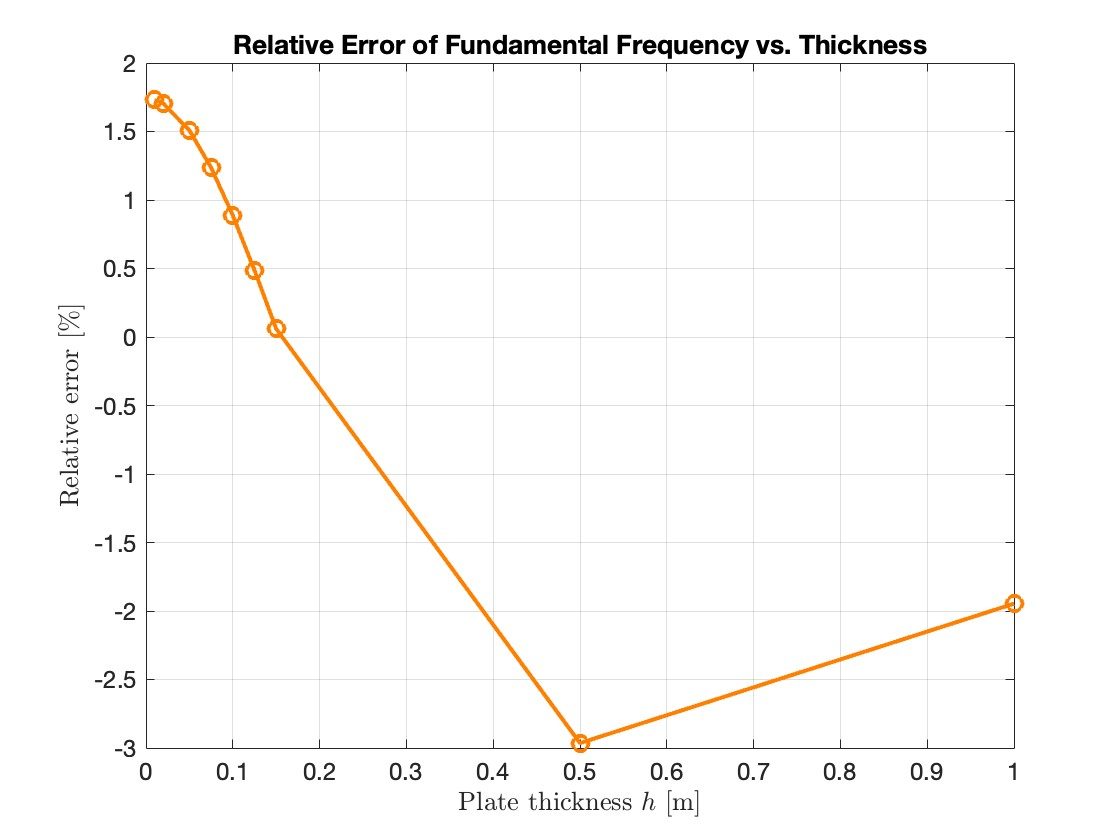
\includegraphics[width=7cm]{../images/errorThickPlates.jpg}
\end{center}

The discrepancy between the exact and approximate fundamental frequencies, especially for very thin or very thick plates, is due to the limitations of the plate theory and finite element modeling assumptions used in the analysis.
\begin{enumerate}
    \item Thin plates (e.g., $h = 0.01$,  $0.02$, $0.05$, $0.075$):  positive relative error, bigger then 1\% (approximate frequency slightly larger than exact).
          \begin{itemize}
              \item In thin plate theory (Kirchhoff-Love), shear deformation is negligible.
              \item However, the numerical model (based on Mindlin theory) still includes shear effects.
              \item  This leads to a small overestimation of first natural frequency.
          \end{itemize}
    \item Moderately thick plates (e.g., $h = 0.1$, $0.125$, $0.15$) : small relative error and good agreement between exact and approximate frequencies.
          \begin{itemize}
              \item The Reissner-Mindlin plate theory, which accounts for transverse shear deformation, is most accurate in this regime.
              \item Both bending and shear effects are significant and correctly captured.
              \item The approximation provided by the numerical method (with appropriate bending and shear stiffness) aligns closely with the exact analytical solution.
          \end{itemize}
    \item  Thick plates and 3d solid ($h = 0.5$ and $0.1$): large negative relative error (approximate frequency much smaller than exact).
          \begin{itemize}
              \item For thick plates, 3D stress states and warping effects become important.
              \item  The plate theory becomes insufficient as it neglects higher-order effects and out-of-plane warping (higher order deformation theory is needed).
              \item  The numerical model underestimates stiffness due to simplifications, leading to an underestimates first frequency.
          \end{itemize}
\end{enumerate}

\end{document}